\definecolor{bgsolved}{HTML}{1F5FA8}
\definecolor{bgfailed}{HTML}{BF8330}
\def\bgcell#1#2#3#4{
    \fill[bg#3] (#1, -#2 - 1) rectangle +(1, 1);
    \fill[bg#4] (#1, -#2 - 1) -- (#1 + 1, -#2 - 1) -- (#1 + 1, -#2) -- cycle;
    \draw[white, line width=0.8pt] (#1, -#2 - 1) rectangle +(1, 1);
}
\def\bgtarget#1#2{\node[anchor=east, font=\footnotesize, inner sep=2pt] at (0, -#1 - 0.5) {#2};}
\def\bgeta#1#2{\node[anchor=base, font=\footnotesize, inner sep=0pt] at (#1 + 0.5, 0.25) {#2};}
\def\bgtitle#1#2{
    \node[anchor=base east, font=\footnotesize, inner sep=2pt] at (0, 0.25) {$\eta$};
    \draw[black!50] (0.1, 1.15) -- (#1 - 0.1, 1.15);
    \node[anchor=south, font=\footnotesize, inner sep=2pt] at (#1 / 2, 1.15) {#2};
}
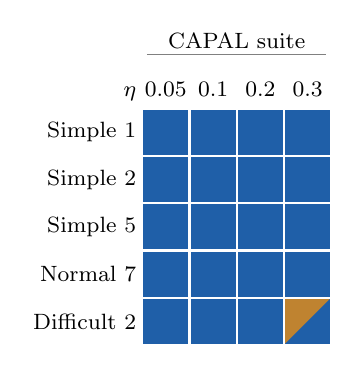
\begin{tikzpicture}[x=0.6cm, y=0.6cm, baseline=0pt]
    \bgtitle{4}{CAPAL suite}
    \bgeta{0}{0.05}
    \bgeta{1}{0.1}
    \bgeta{2}{0.2}
    \bgeta{3}{0.3}
    \bgtarget{0}{Simple 1}
    \bgcell{0}{0}{solved}{solved}
    \bgcell{1}{0}{solved}{solved}
    \bgcell{2}{0}{solved}{solved}
    \bgcell{3}{0}{solved}{solved}
    \bgtarget{1}{Simple 2}
    \bgcell{0}{1}{solved}{solved}
    \bgcell{1}{1}{solved}{solved}
    \bgcell{2}{1}{solved}{solved}
    \bgcell{3}{1}{solved}{solved}
    \bgtarget{2}{Simple 5}
    \bgcell{0}{2}{solved}{solved}
    \bgcell{1}{2}{solved}{solved}
    \bgcell{2}{2}{solved}{solved}
    \bgcell{3}{2}{solved}{solved}
    \bgtarget{3}{Normal 7}
    \bgcell{0}{3}{solved}{solved}
    \bgcell{1}{3}{solved}{solved}
    \bgcell{2}{3}{solved}{solved}
    \bgcell{3}{3}{solved}{solved}
    \bgtarget{4}{Difficult 2}
    \bgcell{0}{4}{solved}{solved}
    \bgcell{1}{4}{solved}{solved}
    \bgcell{2}{4}{solved}{solved}
    \bgcell{3}{4}{failed}{solved}
\end{tikzpicture}
\quad
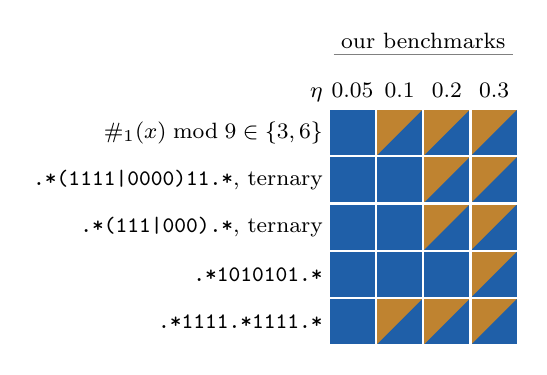
\begin{tikzpicture}[x=0.6cm, y=0.6cm, baseline=0pt]
    \bgtitle{4}{our benchmarks}
    \bgeta{0}{0.05}
    \bgeta{1}{0.1}
    \bgeta{2}{0.2}
    \bgeta{3}{0.3}
    \bgtarget{0}{$\#_1(x) \bmod 9 \in \{3, 6\}$}
    \bgcell{0}{0}{solved}{solved}
    \bgcell{1}{0}{failed}{solved}
    \bgcell{2}{0}{failed}{solved}
    \bgcell{3}{0}{failed}{solved}
    \bgtarget{1}{\texttt{.*(1111|0000)11.*}, ternary}
    \bgcell{0}{1}{solved}{solved}
    \bgcell{1}{1}{solved}{solved}
    \bgcell{2}{1}{failed}{solved}
    \bgcell{3}{1}{failed}{solved}
    \bgtarget{2}{\texttt{.*(111|000).*}, ternary}
    \bgcell{0}{2}{solved}{solved}
    \bgcell{1}{2}{solved}{solved}
    \bgcell{2}{2}{failed}{solved}
    \bgcell{3}{2}{failed}{solved}
    \bgtarget{3}{\texttt{.*1010101.*}}
    \bgcell{0}{3}{solved}{solved}
    \bgcell{1}{3}{solved}{solved}
    \bgcell{2}{3}{solved}{solved}
    \bgcell{3}{3}{failed}{solved}
    \bgtarget{4}{\texttt{.*1111.*1111.*}}
    \bgcell{0}{4}{solved}{solved}
    \bgcell{1}{4}{failed}{solved}
    \bgcell{2}{4}{failed}{solved}
    \bgcell{3}{4}{failed}{solved}
\end{tikzpicture}
\quad
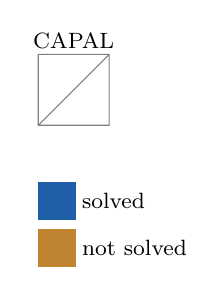
\begin{tikzpicture}[x=0.6cm, y=0.6cm, baseline=0pt, font=\footnotesize]
    \draw[black!50] (0, -1.5) rectangle (1.5, 0) (0, -1.5) -- (1.5, 0);
    \node[anchor=south, inner sep=2pt] at (0.75, 0) {CAPAL};
    \node[anchor=north, inner sep=2pt] at (0.75, -1.5) {\ours{}};
    \foreach \kind/\name [count=\i] in {solved/solved, failed/not solved} {
        \fill[bg\kind] (0, -2.5 - \i) rectangle +(0.8, 0.8);
        \node[anchor=west, inner sep=2pt] at (0.8, -2.1 - \i) {\name};
    }
\end{tikzpicture}
